\documentclass{article}
\usepackage[utf8]{inputenc}
\usepackage[spanish]{babel}
\usepackage{listings}
\usepackage{graphicx}
\graphicspath{ {images/} }
\usepackage{cite}

\begin{document}

\begin{titlepage}
    \begin{center}
        \vspace*{1cm}
            
        \Huge
        \textbf{Tarea 1}
            
        \vspace{0.5cm}
        \LARGE
        
            
        \vspace{1.5cm}
            
        \textbf{Julián David Londoño Pamplona}
            
        \vfill
            
        \vspace{0.8cm}
            
        \Large
        Despartamento de Ingeniería Electrónica y Telecomunicaciones\\
        Universidad de Antioquia\\
        Medellín\\
        Marzo de 2021
            
    \end{center}
\end{titlepage}

\tableofcontents
\newpage
\section{Descripción}\label{intro}
El punto de partida constará de una hoja de papel, dos cartas y una superficie para trabajar.

\section{Estado inicial} \label{contenido}
La hoja inicialmente debe estar sobre la mesa, y sobre esta las dos cartas, como se muestra en la imagen 1.
\begin{figure}[h]
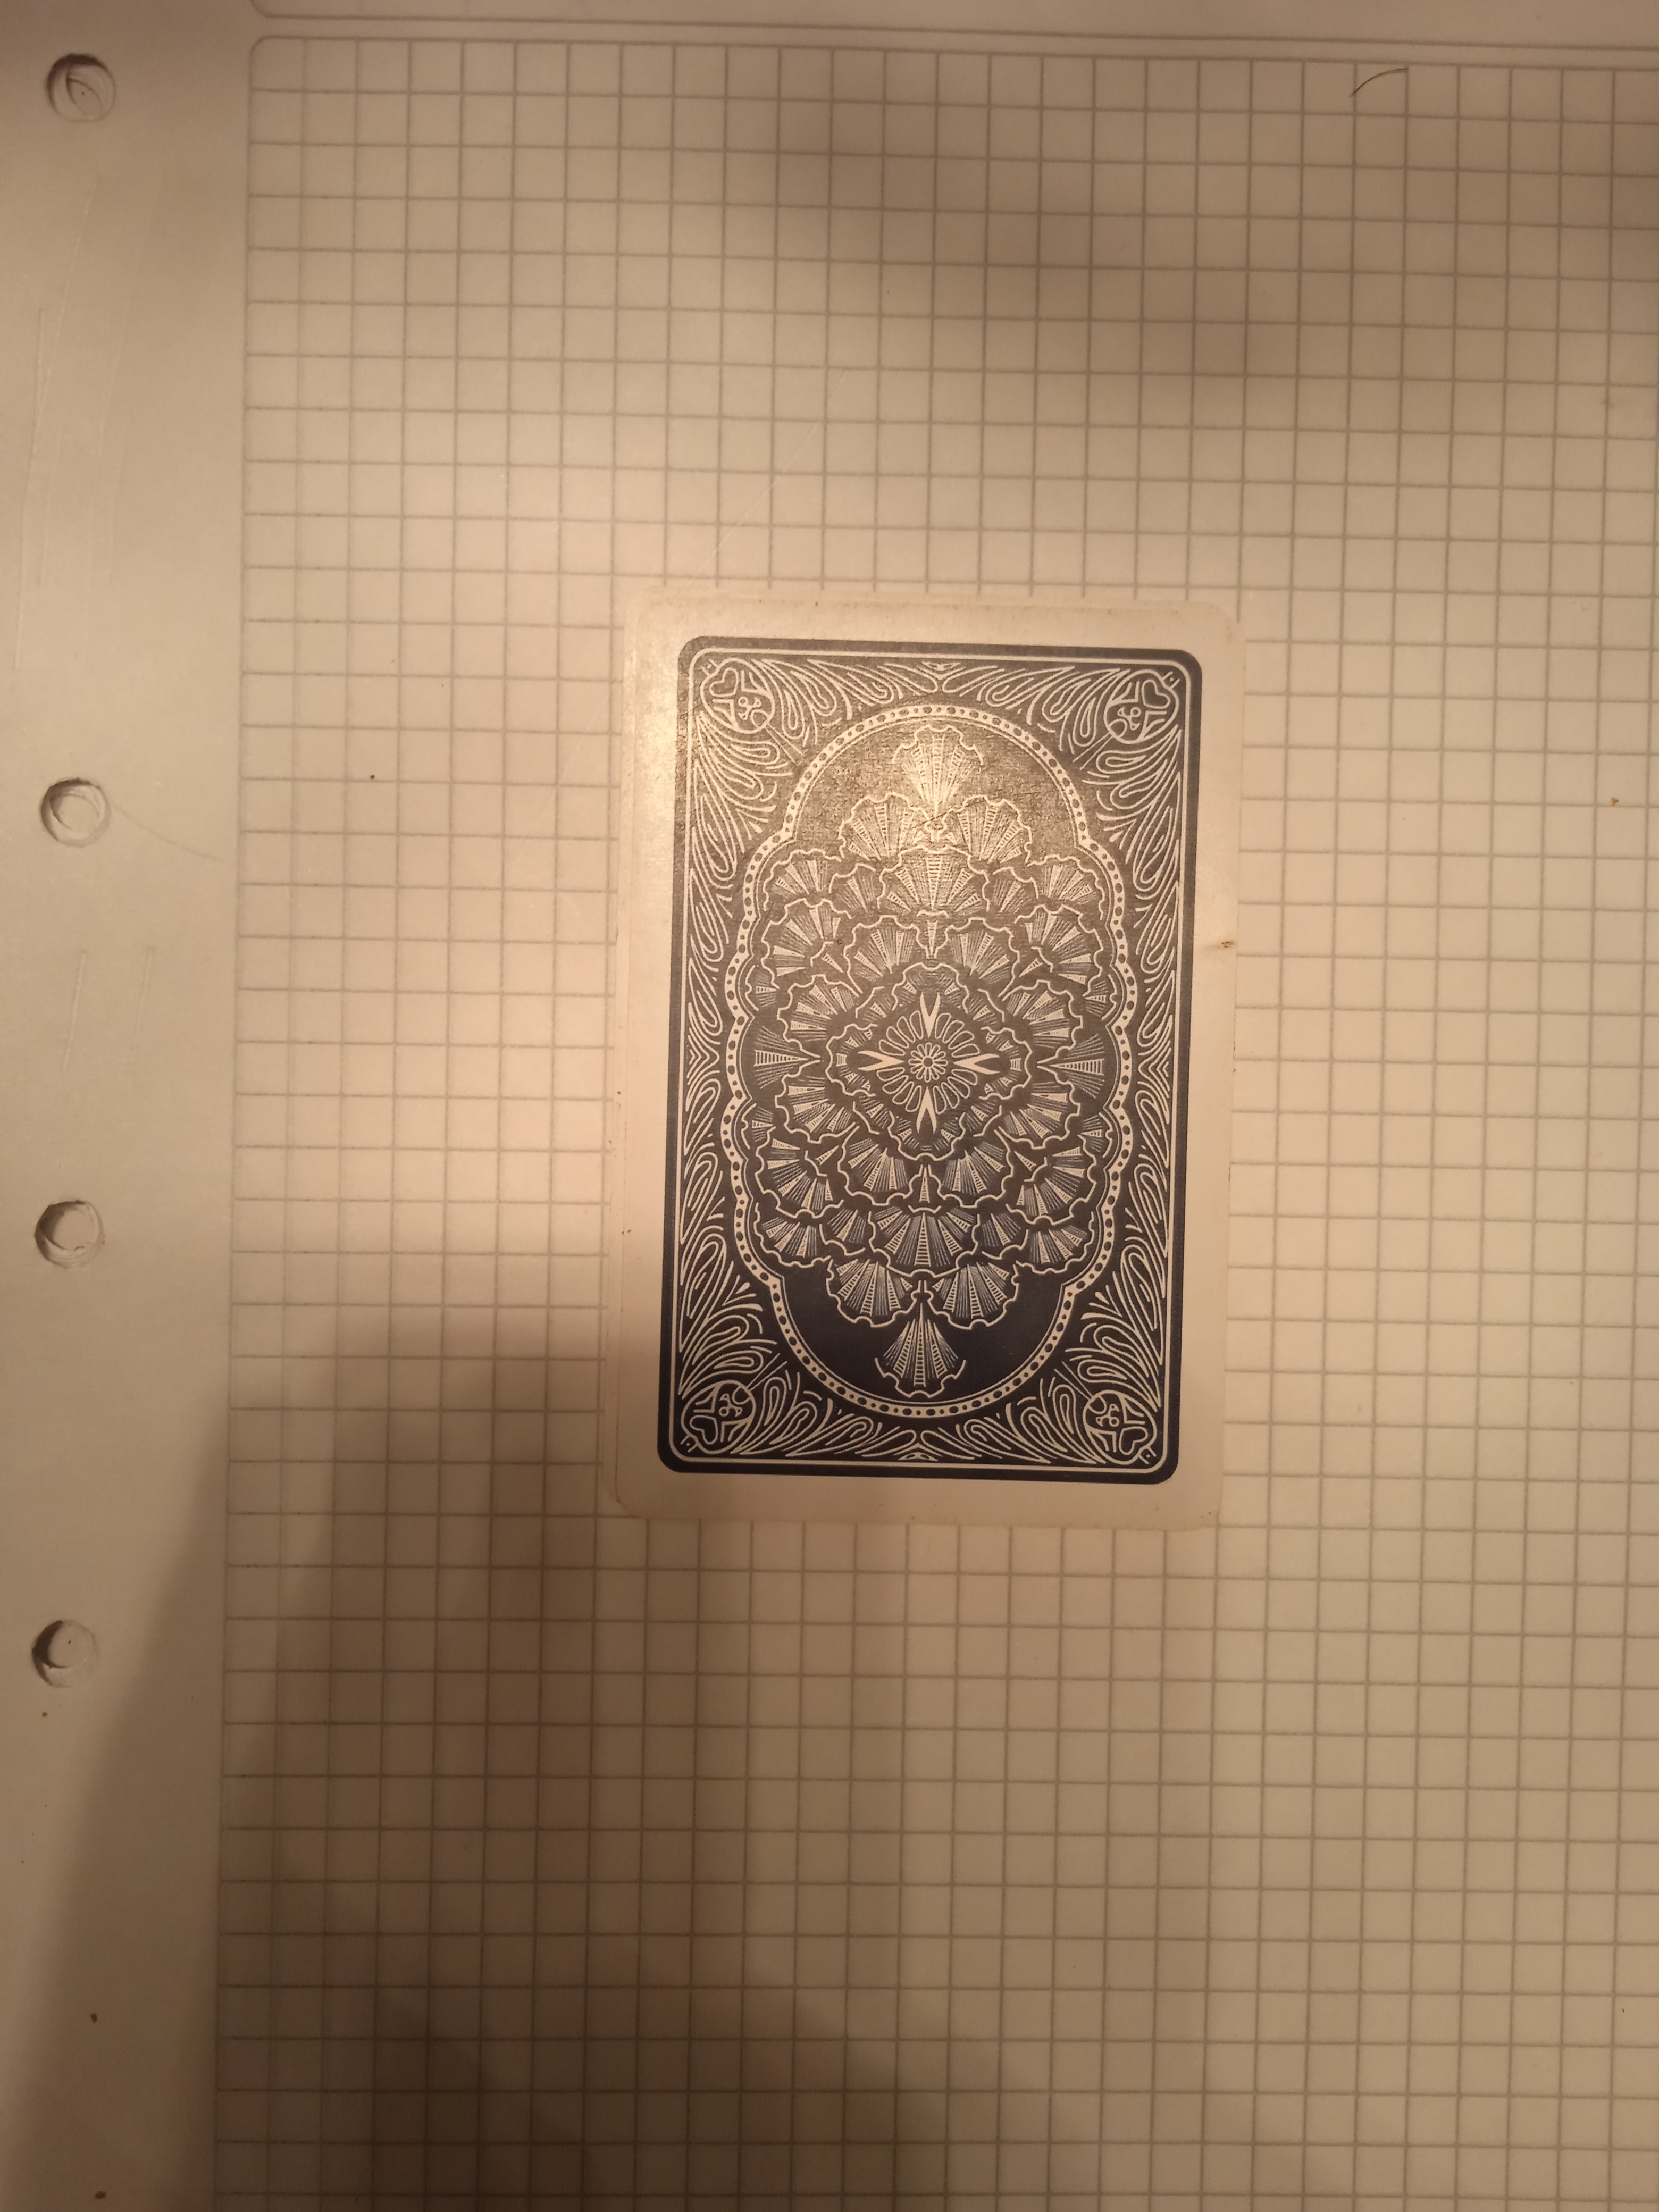
\includegraphics[width=4cm]{imagen 1.png}
\centering
\caption{imagen 1}
\label{fig:cpplogo}
\end{figure}

\section{Paso a paso} \label{contenido}
Se deben tomar las cartas por uno de sus bordes mas cortos, sosteniendo las dos puntas de ese borde, vea la imagen 2. 

\\

\begin{figure}[h]
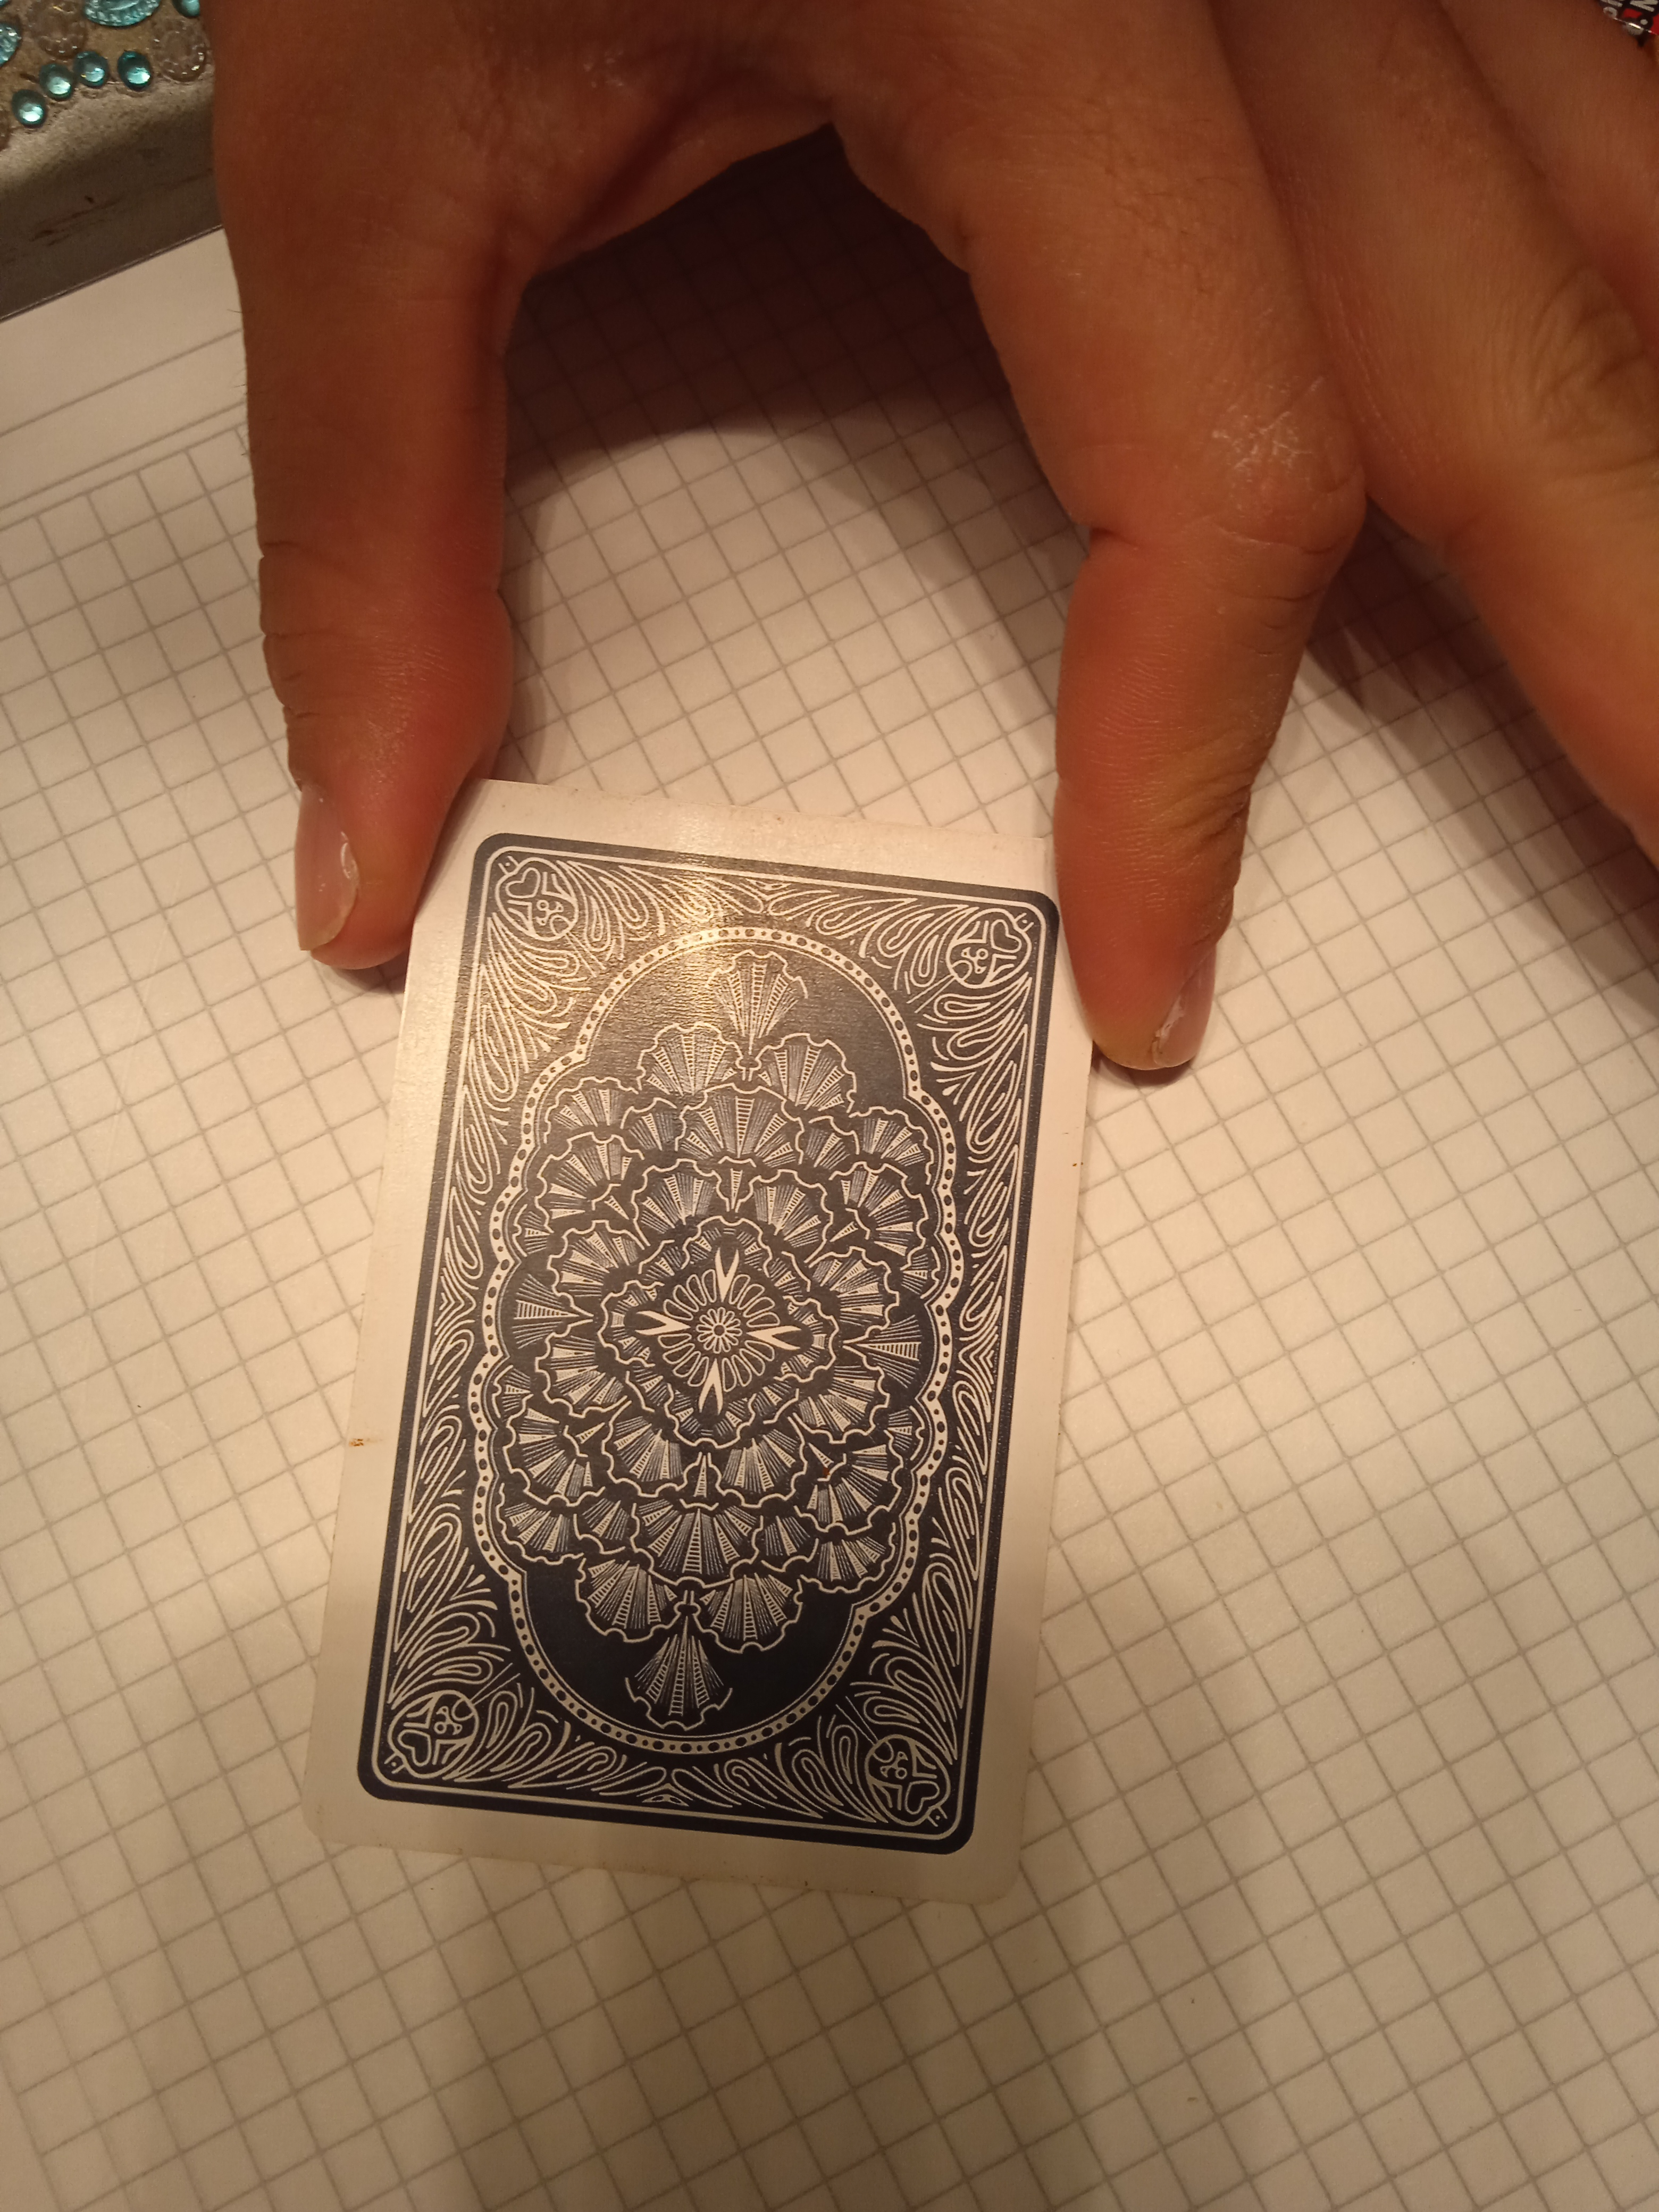
\includegraphics[width=4cm]{imagen 2.png}
\centering
\caption{imagen 2}
\label{fig:cpplogo}
\end{figure}
\\
Se levantan las cartas de manera vertical sobre la hoja, alzarlas unos 3 cm, separar las cartas usando un dedo como se muestra en la imagen 3,
\\
\begin{figure}[h]
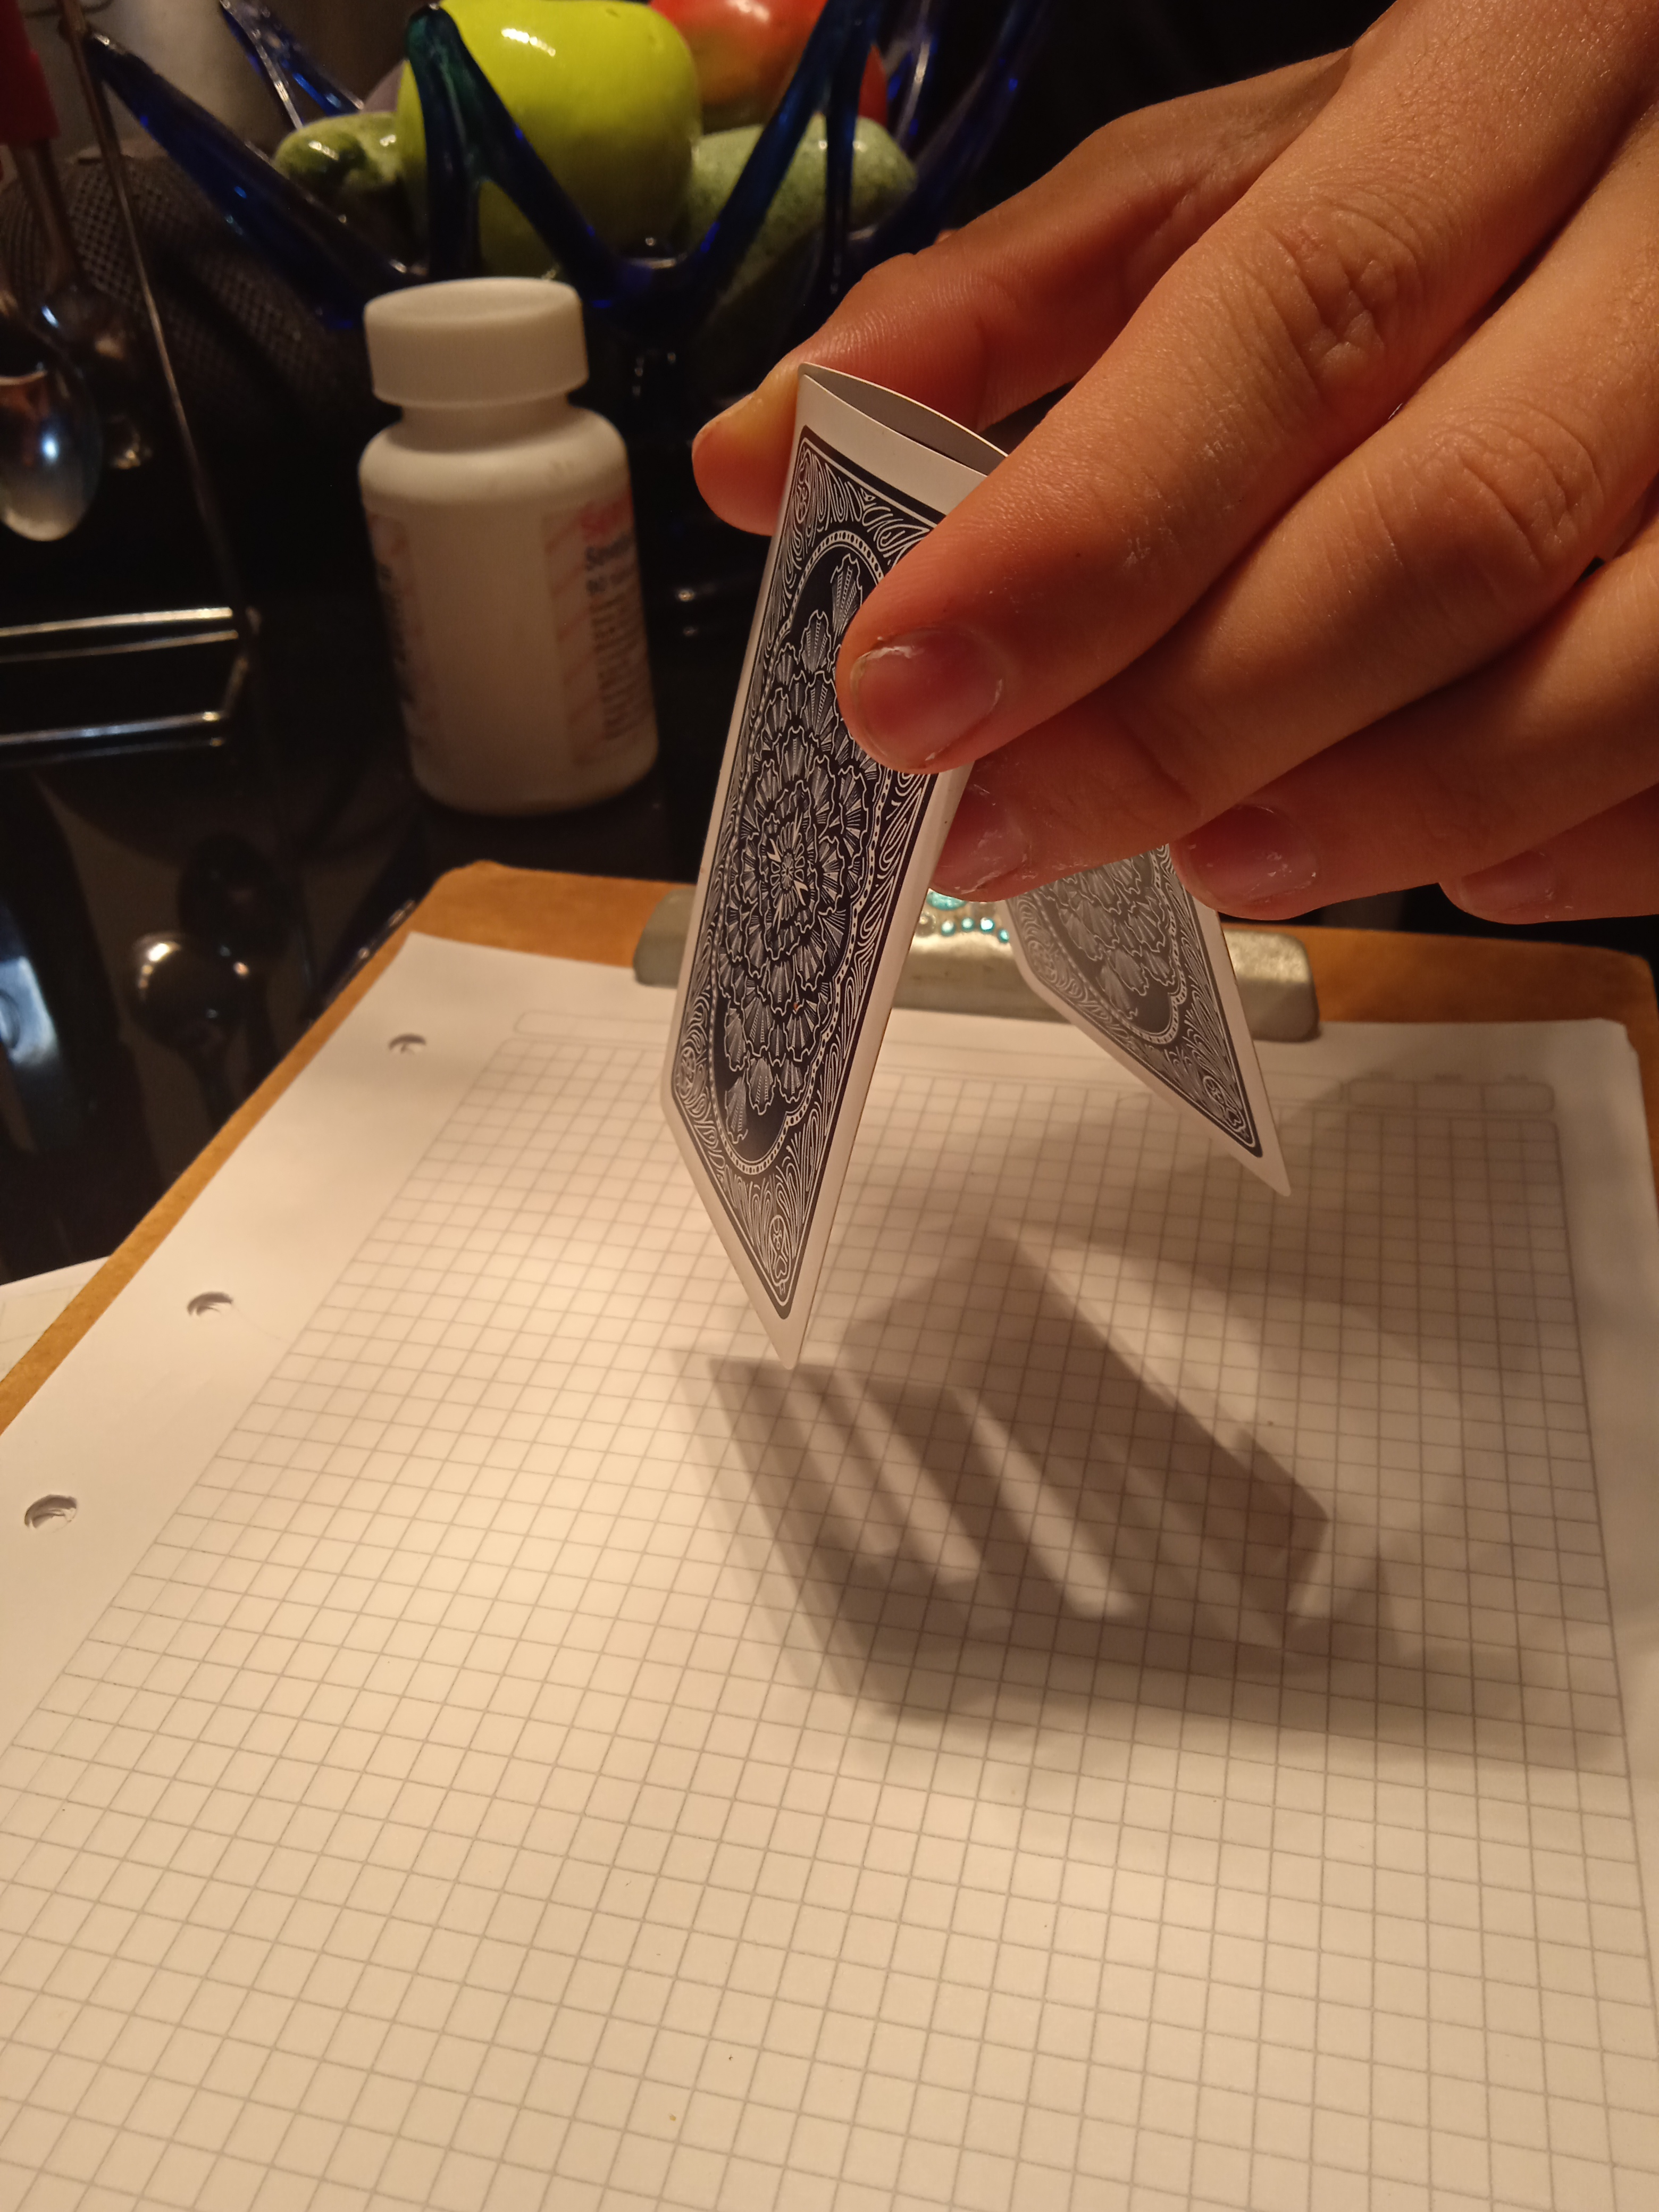
\includegraphics[width=4cm]{imagen 3.png}
\centering
\caption{imagen 3}
\label{fig:cpplogo}
\end{figure}
\\
las cartas deben permanecer unidas en el borde en donde se tomaron, y una de las cartas se debe elevar hasta unos 30 grados aproximadamente de su posición original mientras la otra permanece vertical, bajar las cartas hasta que el borde corto, del que no está sujeta la carta que aun se encuentra completamente vertical, toque la hoja, vea la imagen 4.
\\
\begin{figure}[h]
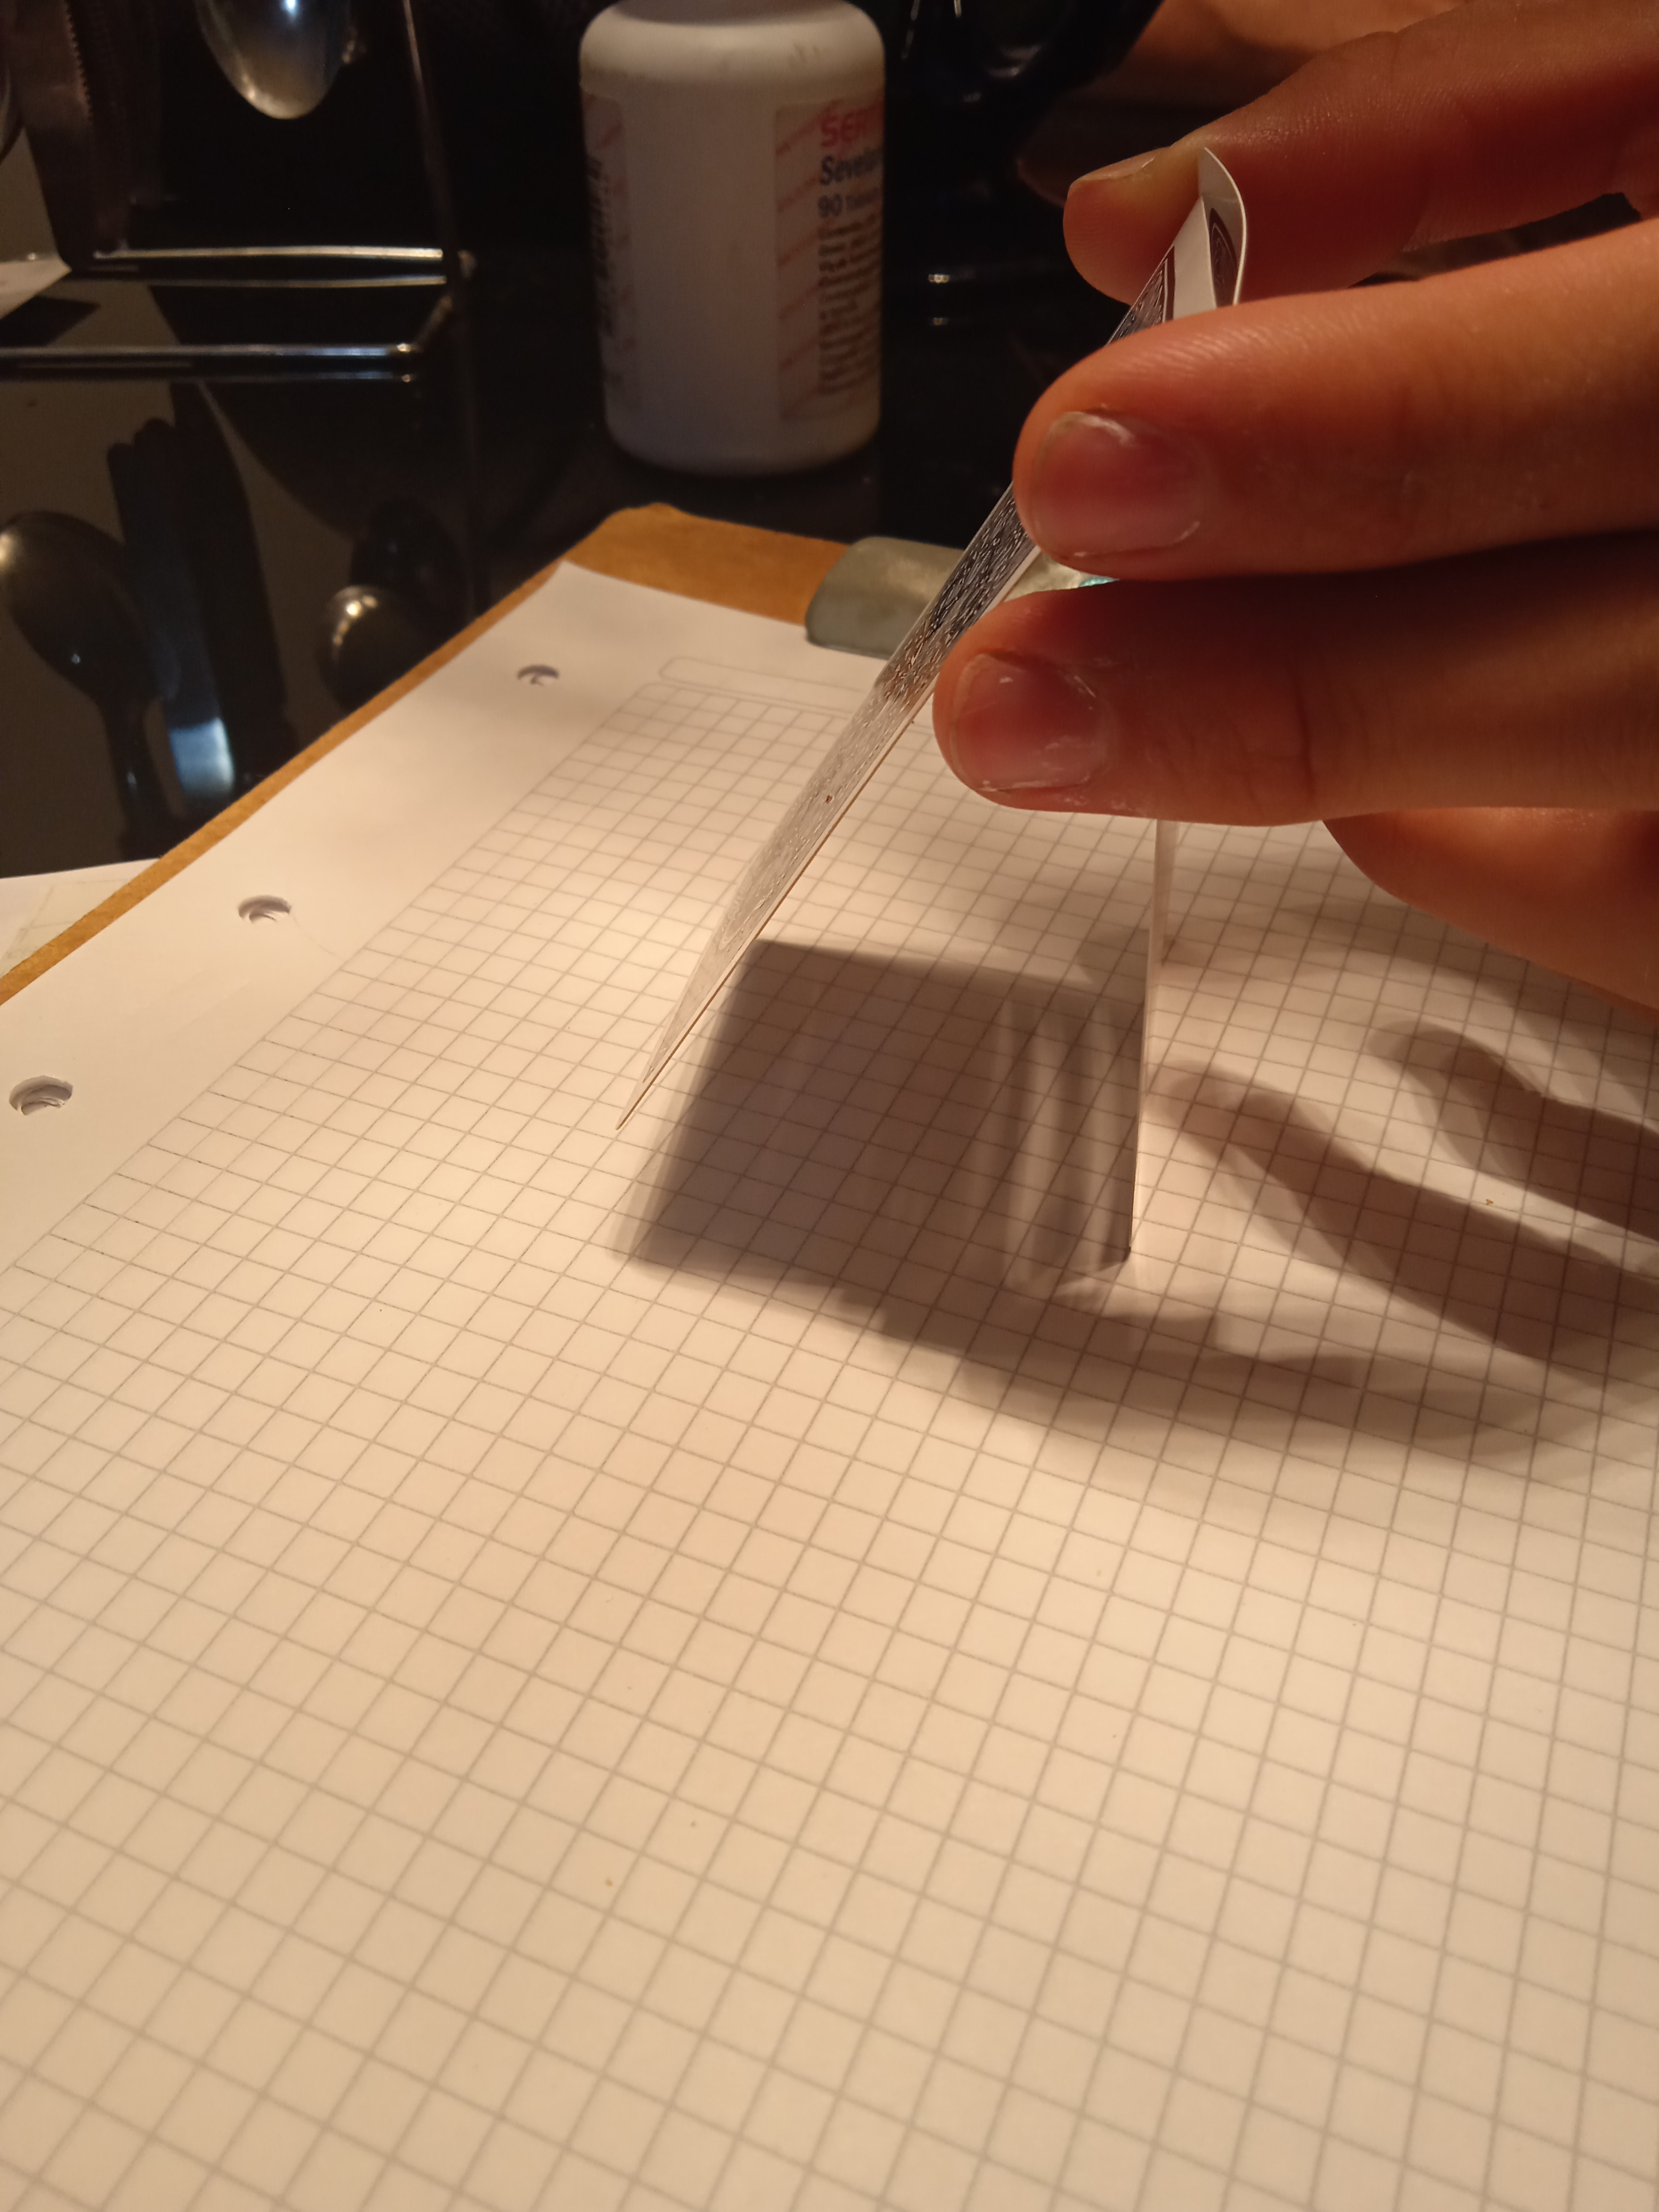
\includegraphics[width=4cm]{imagen 4.png}
\centering
\caption{imagen 4}
\label{fig:cpplogo}
\end{figure}
\\
La carta que aun se encuentra en el aire debe tocar la superficie de la hoja, en frente a la que inicialmente tocó la hoja a unos 5 cm como se muestra en la imagen, y estabilizar las cartas hasta que las cartas queden paradas  por si solas como se muestra en la imagen 6.
\\
\begin{figure}[h]
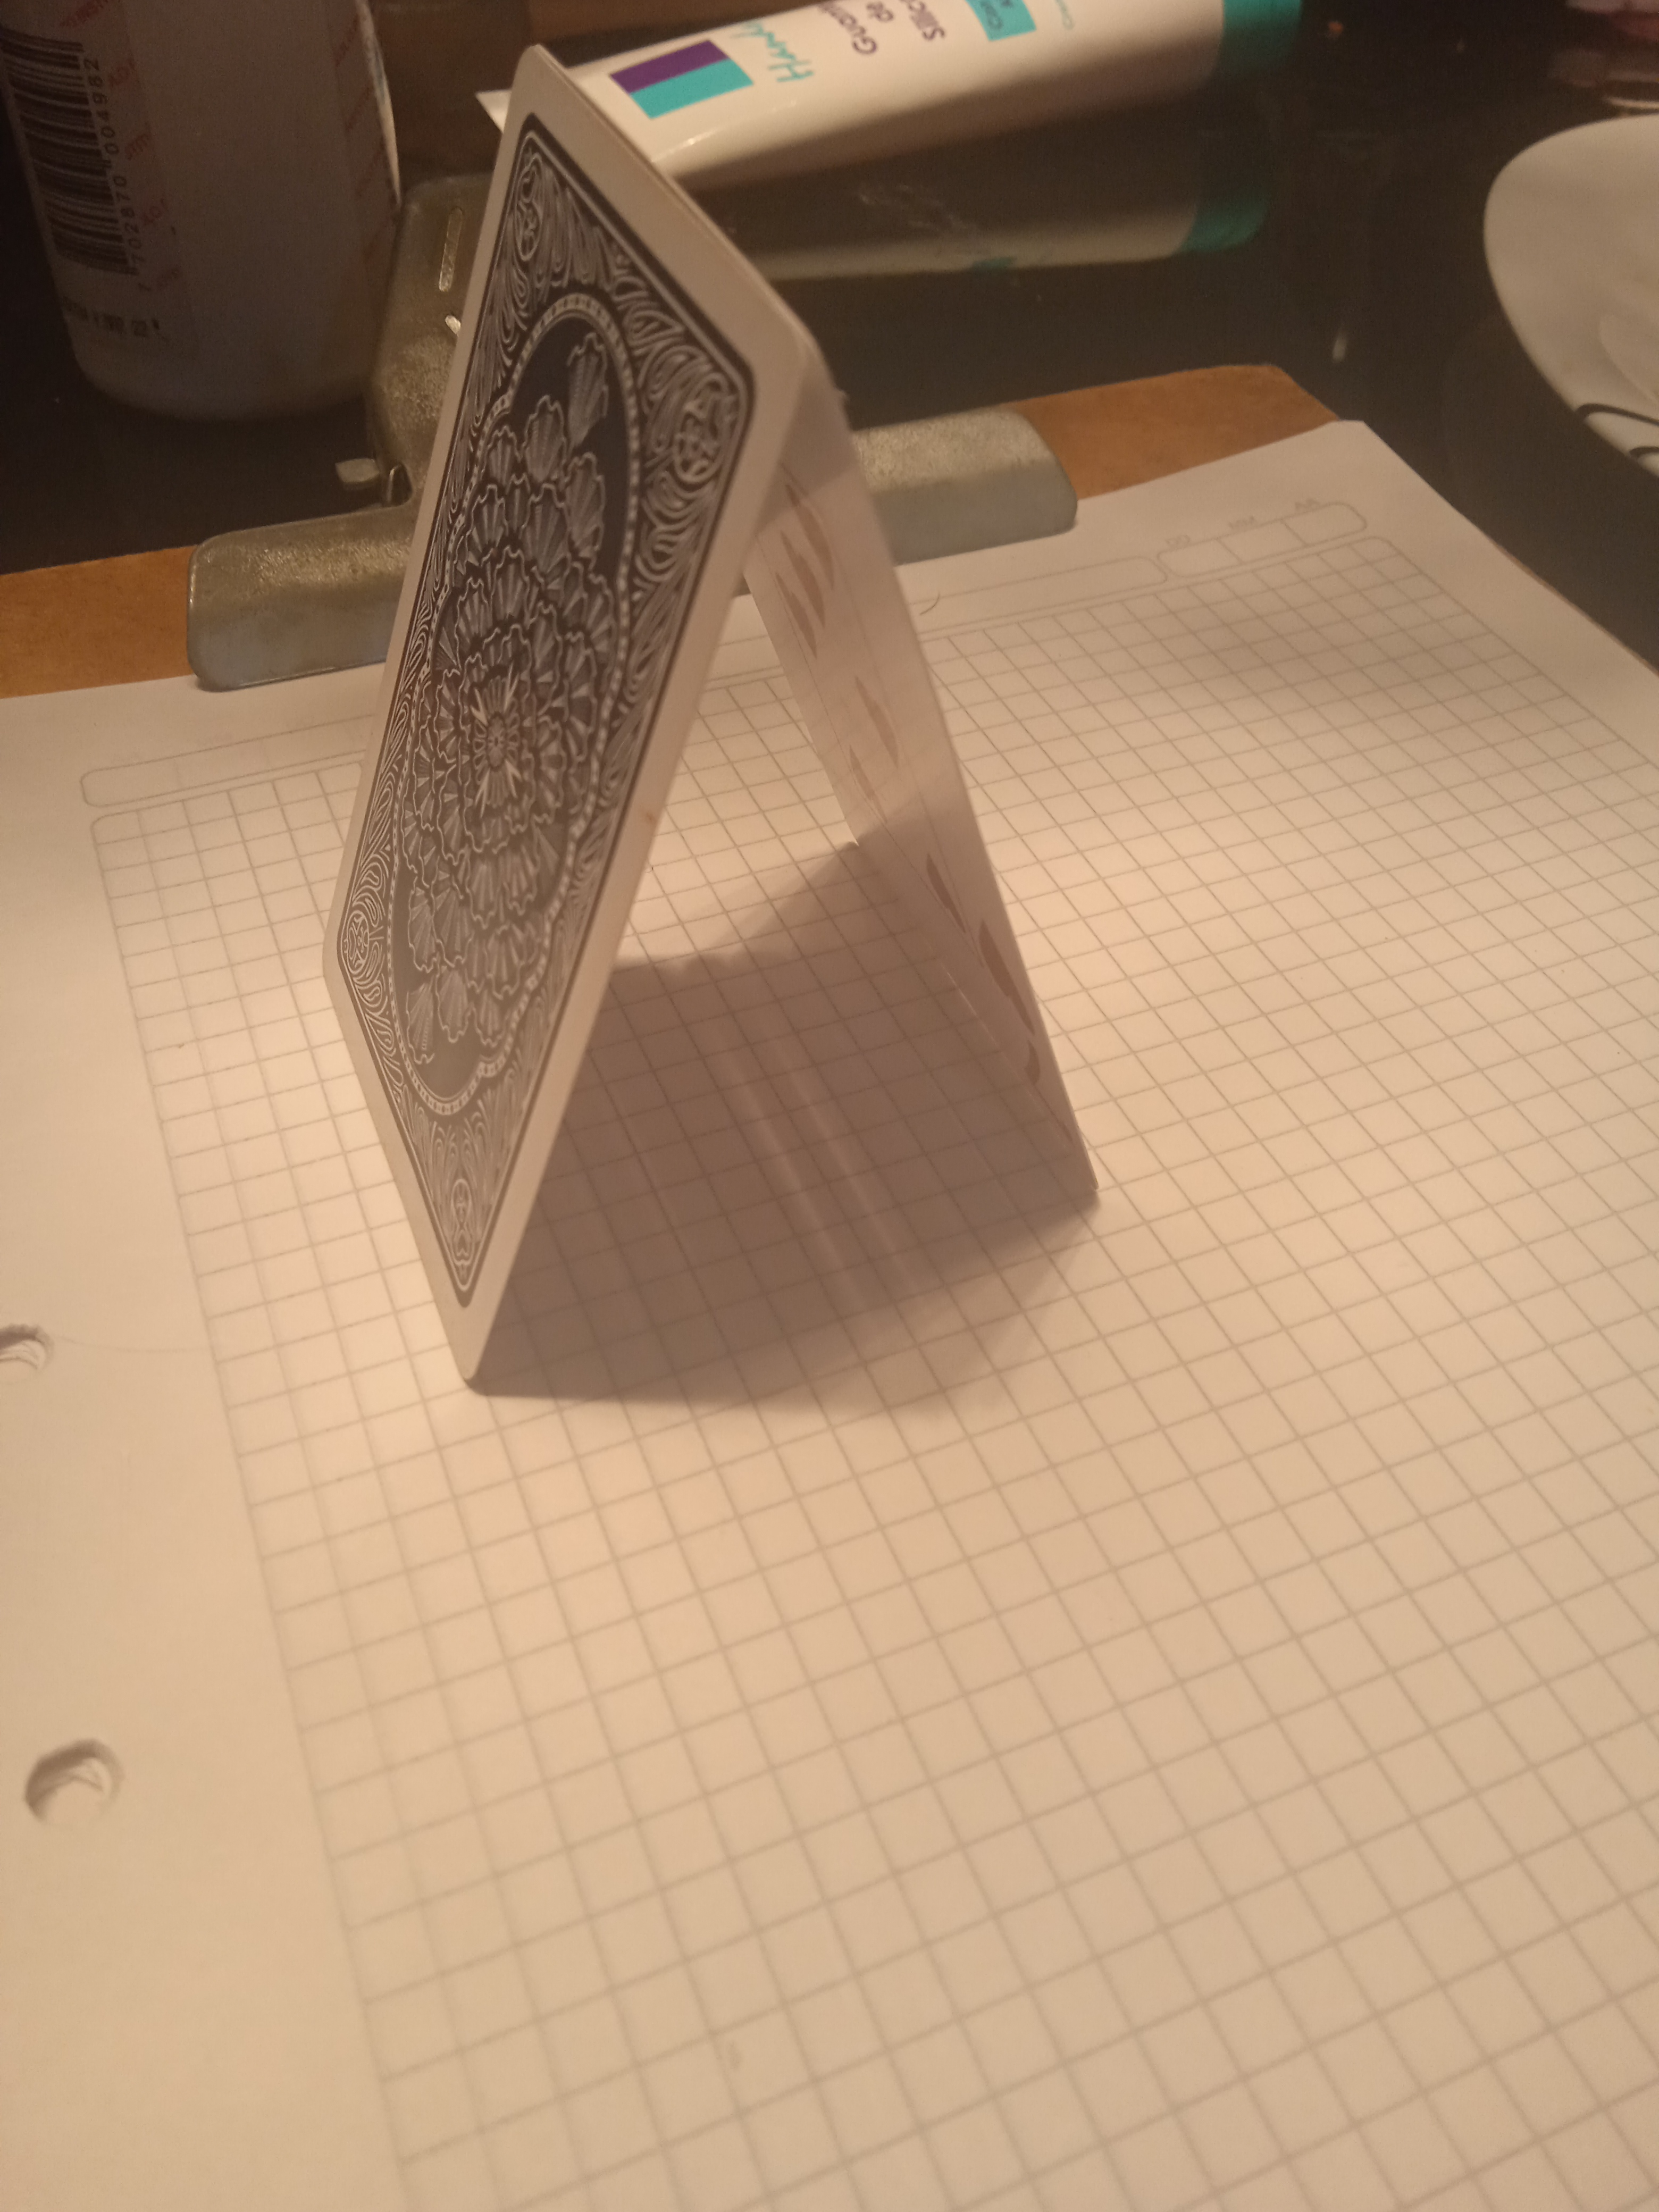
\includegraphics[width=4cm]{imagen 6.png}
\centering
\caption{imagen 6}
\label{fig:cpplogo}
\end{figure}
\\








\end{document}
